
\chapter{Examples}\label{chap2}

WE\pageoriginale GIVE IN this section several examples of the abstract
problem formulated in Sec.~\ref{chap1}. We interpret the solutions of these
problems as solutions of classical boundary value problems which often
occur in the theory of Elasticity.

Before we proceed with the examples, we summarize briefly the results
(without proofs) on Sobolev spaces which will prove to be very useful
in our discussion.

Henceforth $\Omega\subset \mathbb{R}^{n}$ will denote an open set
(more often $\Omega$ will be a bounded open set with a specific type
of boundary which will be described presently). A {\em multi-index}
$\alpha$ will denote an $n$-tuple $(\alpha_{1},\ldots,\alpha_{n})$ of
non-negative integers, and we denote 
\begin{equation*}
|\alpha|=\alpha_{1}+\cdots+\alpha_{n},\tag{2.1}\label{chap2-eq2.1} 
\end{equation*}
and call it the {\em length} of the multi-index. If $v$ is a
real-valued function on $\Omega$ for which all derivatives upto order
$m$ exist, for a multi-index $\alpha$ with $|\alpha|\leq m$ we define
\begin{equation*}
\partial^{\alpha_{v}}=\frac{\partial^{|\alpha|_{v}}}{\partial^{\alpha_{1}}_{x_{1}}\ldots
  \partial^{\alpha_{n}}_{x_{n}}}. \tag{2.2}\label{chap2-eq2.2}
\end{equation*}

The space of {\em test functions} on $\Omega$ is given by
\begin{equation*}
\mathscr{D}(\Omega)=\left\{v\in C^{\infty}(\Omega);\supp(v)\text{~ is
  a compact subset of~ }\Omega\right\}.\tag{2.3}\label{chap2-eq2.3}
\end{equation*}
where
\begin{equation*}
\supp (v)=\overline{\{x\in\Omega; v(x)\neq
  0\}}.\tag{2.4}\label{chap2-eq2.4} 
\end{equation*}

\begin{definition}\label{chap2-def2.1}
Let\pageoriginale $m\geq 0$ be an integer. Then the Sobolev space
$H^{m}(\Omega)$ is given by
\begin{equation*}
H^{m}(\Omega)=\left\{v\in L^{2}(\Omega);\partial^{\alpha}v\in
L^{2}(\Omega)~\text{ for all }~ |\alpha|\leq
  m\right\},\tag{2.5}\label{chap2-eq2.5} 
\end{equation*}
where all derivatives are understood in the sense of distributions.
\end{definition}

On $H^{m}(\Omega)$ one can define a norm by means of the formula
\begin{equation*}
||v||_{m,\Omega}=\left(\sum_{|\alpha|\leq
  m}\int_{\Omega}|\partial^{\alpha}v|^{2}dx\right)^{\frac{1}{2}},\quad
v\in H^{m}(\Omega).\tag{2.6}\label{chap2-eq2.6} 
\end{equation*}

It is easy to check that $||\cdot ||_{m,\Omega}$ defines a norm on
$H^{m}(\Omega)$, which makes it a Hilbert space. One can also define a
semi-norm by
\begin{equation*}
|v|_{m,\Omega}=\left(\sum_{|\alpha|=m}\int_{\Omega}|\partial^{\alpha}v|^{2}dx\right)^{\frac{1}{2}},\quad
v\in H^{m}(\Omega).\tag{2.7}\label{chap2-eq2.7}
\end{equation*}

Note that since for all $m\geq 0$, $\mathscr{D}(\Omega)\subset
H^{m}(\Omega)$, we may define,
\begin{equation*}
H^{m}_{0}(\Omega)=\overline{\mathscr{D}(\Omega)},\tag{2.8}\label{chap2-eq2.8} 
\end{equation*}
the closure being taken with respect to the topology of
$H^{m}(\Omega)$. Since $H^{m}_{0}(\Omega)$ is a closed subspace of
$H^{m}(\Omega)$, it is also a Hilbert space under the restriction of
the norm $||\cdot||_{m,\Omega}$. We also have a stronger result:

\begin{theorem}\label{chap2-thm2.1}
Assume that $\Omega$ is a bounded open set. Then over
$H^{m}_{0}(\Omega)$ the semi-norm $|\cdot|_{m,\Omega}$ is a norm
equivalent to the norm $||\cdot||_{m,\Omega}$.
\end{theorem}

This result is a consequence of the following:

\begin{theorem}[POINCAR\'E-FRIEDRICHS' INEQUALITY]\label{chap2-thm2.2}
If $\Omega$ is a bounded open set, there exists a constant
$C=C(\Omega)$ such that, for all $v\in H^{1}_{0}(\Omega)$,
\begin{equation*}
|v|_{0,\Omega}\leq C|v|_{1,\Omega}.\tag{2.9}\label{chap2-eq2.9}
\end{equation*}
\end{theorem}

Henceforth,\pageoriginale unless specified to the contrary, the
following will be our standing assumptions: $\Omega$ {\em is a bounded
  open subset of $\mathbb{R}^{n}$. If $\Gamma$ is the boundary of
  $\Omega$, then $\Gamma$ is Lipschitz continuous in the sense of
  Ne\v{c}as} \cite{key20}. (Essentially, $\Gamma$ can be covered by a
  finite number of local coordinate systems, such that in each, the
  corresponding portion of $\Gamma$ is described by a Lipschitz
  continuous function).

If $L^{2}(\Gamma)$ is defined in the usual fashion using the Lipschitz
continuity of $\Gamma$, one has the following result:

\begin{theorem}\label{chap2-thm2.3}
There exists a constant $C=C(\Omega)$ such that, for all $v\in
C^{\infty}(\Omega)$, 
\begin{equation*}
||v||_{L^{2}(\Omega)}\leq
C||v||_{1,\Omega}.\tag{2.10}\label{chap2-eq2.10} 
\end{equation*}
\end{theorem}

By virtue of Theorem \ref{chap2-thm2.3} we get that if $v\in
C^{\infty}(\overline{\Omega})$, then its restriction to $\Gamma$ is an
element of $L^{2}(\Gamma)$. Thus we have a map from the space
$C^{\infty}(\overline{\Omega})$ equipped with the norm $||\cdot
||_{1,\Omega}$ into the space $L^{2}(\Gamma)$ which is continuous. We
also have:

\begin{theorem}\label{chap2-thm2.4}
The space $C^{\infty}(\overline{\Omega})$ is dense in $H^{1}(\Omega)$,
for domains with Lipschitz continuous boundaries.
\end{theorem}

Consequently, the above map may be extended to a continuous map
$H^{1}(\Omega)\to L^{2}(\Gamma)$ which we denote by $\tr_{\Gamma}$. It
is called the {\em trace operator}. An important result on the trace is
the characterization:
\begin{equation*}
H^{1}_{0}(\Omega)=\left\{v\in
H^{1}(\Omega);\ \tr_{\Gamma}v=0\right\}.\tag{2.11}\label{chap2-eq2.11} 
\end{equation*}

When no confusion is likely to occur we will merely write $v$ instead
of $\tr_{\Gamma}v$. In fact if $v$ is a ``smooth'' function then
$\tr_{\Gamma}v$ is the restriction of $v$ to $\Gamma$. 

Retaining\pageoriginale our assumption on $\Omega$ and $\Gamma$, the
unit outer normal $\overrightarrow{\nu}$ is defined a.e.\@ on
$\Gamma$. Let $\overrightarrow{\nu}=(\nu_1,\ldots,\nu_{n})$. If $v$ is
smooth then we may define the {\em outer normal derivative}
$\dfrac{\partial {\rm v}}{\partial \nu}$ by
\begin{equation*}
\frac{\partial {\rm v}}{\partial \nu}=\sum^{n}_{i=1}\nu_{i}\frac{\partial
  {\rm v}}{\partial x_{i}}.\tag{2.12}\label{chap2-eq2.12}
\end{equation*}

We extend this definition to $v\in H^{2}(\Omega)$. If $v\in
H^{2}(\Omega)$, then $\dfrac{\partial v}{\partial x_{i}}\in
H^{1}(\Omega)$ and hence $\tr_{\Gamma}\dfrac{\partial v}{\partial
  x_{i}}\in L^{2}(\Gamma)$. We now define
\begin{equation*}
\frac{\partial v}{\partial
  \nu}=\sum^{n}_{i=1}\nu_{i}\tr_{\Gamma}\frac{\partial v}{\partial
  x_{i}}.\tag{2.13}\label{chap2-eq2.13} 
\end{equation*}

However when there is no confusion we write it in the form of
\eqref{chap2-eq2.12}. Then one has the following characterization:
\begin{equation*}
H^{2}_{0}(\Omega)=\left\{v\in H^{2}(\Omega);\ v=\frac{\partial
  v}{\partial\nu}=0\text{~ on~
}\Gamma\right\}.\tag{2.14}\label{chap2-eq2.14} 
\end{equation*}

\begin{theorem}[GREEN'S FORMULA IN SOBOLEV SPACES]\label{chap2-thm2.5}
Let $u$, $v\in H^{1}(\Omega)$. Then we have
\begin{equation*}
\int_{\Omega}u\frac{\partial v}{\partial
  x_{i}}dx=-\int_{\Omega}\frac{\partial u}{\partial
  x_{i}}v\ dx+\int_{\Gamma}u\ v\nu_{i} \; d\gamma,\tag{2.15}\label{chap2-eq2.15} 
\end{equation*}
for all $1\leq i\leq n$.
\end{theorem}

If we assume $u\in H^{2}(\Omega)$, we may replace $u$ in
\eqref{chap2-eq2.15} by $\dfrac{\partial u}{\partial x_{i}}$; summing
over all $1\leq i\leq n$, we get for $u\in H^{2}(\Omega)$, $v\in
H^{1}(\Omega)$, 
\begin{equation*}
\int_{\Omega}\sum^{n}_{i=1}\frac{\partial u}{\partial
  x_{i}}\frac{\partial v}{\partial x_{i}}dx=-\int_{\Omega}\Delta
u\ v\ dx+\int_{\Omega}\frac{\partial u}{\partial
  \nu}v\ d\gamma,\tag{2.16}\label{chap2-eq2.16} 
\end{equation*}
where $\Delta=\sum^{n}_{i=1}\frac{\partial^{2}}{\partial x^{2}_{i}}$
is the Laplacian.

If both $u$ and $v$ are in $H^{2}(\Omega)$, we may interchange the
roles of $u$ and $v$ in \eqref{chap2-eq2.16}. Subtracting one formula
from the other, we get 
\begin{equation*}
\int_{\Omega}(u\Delta v-\Delta uv)dx=\int_{\Gamma}\left(u\frac{\p
  v}{\p \nu}-\frac{\p u}{\p
  \nu}v\right)d\gamma,\tag{2.17}\label{chap2-eq2.17} 
\end{equation*}\pageoriginale
for $u$, $v\in H^{2}(\Omega)$.

Finally replacing $u$ by $\Delta u$ in \eqref{chap2-eq2.17} we get,
for $u\in H^{4}(\Omega)$, $v\in H^{2}(\Omega)$,
\begin{equation*}
\int_{\Omega}\Delta u\Delta
v\ dx=\int_{\Omega}\Delta^{2}u\ v\ dx+\int_{\Gamma}\Delta u\frac{\p
  v}{\p \nu}d\gamma-\int_{\Gamma}\frac{\p(\Delta u)}{\p
  \nu}vd\gamma.\tag{2.18}\label{chap2-eq2.18} 
\end{equation*}

The formulae \eqref{chap2-eq2.15} through \eqref{chap2-eq2.18} are all
known as {\em Green's formulae} in Sobolev spaces.

We derive two results from these formulae. These results will be
useful later.

\begin{lemma}\label{chap2-lem2.1}
For all $v\in H^{2}_{0}(\Omega)$,
\begin{equation*}
|\Delta v|_{0,\Omega}=|v|_{2,\Omega}.\tag{2.19}\label{chap2-eq2.19}
\end{equation*}

Consequently over $H^{2}_{0}(\Omega)$, the mapping $v\mapsto |\Delta
v|_{0,\Omega}$ is a norm equivalent to the norm $||\cdot ||_{2,\Omega}$.
\end{lemma}

\begin{proof}
Since $\mathscr{D}(\Omega)$ is dense in $H^{2}_{0}(\Omega)$, it
suffices to prove \eqref{chap2-eq2.19} for
$v\in\mathscr{d}(\Omega)$. Let $v\in\mathscr{D}(\Omega)$. Then
$$
|\Delta v|^{2}=\sum^{n}_{i=1}\left(\frac{\p^{2}v}{\p
  x^{2}_{i}}\right)^{2}+2\sum_{1\leq i<j\leq n}\frac{\p^{2}v}{\p
  x^{2}_{i}}\frac{\p^{2}v}{\p x^{2}_{j}}. 
$$

By Green's formula \eqref{chap2-eq2.15},
\begin{equation*}
\int_{\Omega}\frac{\p^{2}v}{\p x^{2}_{i}}\frac{\p^{2}v}{\p
  x^{2}_{j}}dx=-\int_{\Omega} \frac{\p v}{\p x_{i}}\frac{\p^{3}v}{\p
  x_{i}\p x^{2}_{j}}dx=\int_{\Omega}\left(\frac{\p^{2}v}{\p x_{i}\p
  x_{j}}\right)^{2}dx\tag{2.20}\label{chap2-eq2.20} 
\end{equation*}
for, the integrals over $\Gamma$ vanish for
$v\in\mathscr{D}(\Omega)$. (cf. \eqref{chap2-eq2.11}). Now
\eqref{chap2-eq2.19} follows directly from \eqref{chap2-eq2.20}. This
proves the lemma.
\end{proof}

\begin{lemma}\label{chap2-lem2.2}
Let\pageoriginale $\Omega\subset\mathbb{R}^{2}$. Then for $u\in H^{3}(\Omega)$,
$v\in H^{2}(\Omega)$,
\begin{equation*}
\begin{split}
& \int_{\Omega}2\frac{\p^{2}u}{\p x_{1}\p x_{2}}\frac{\p^{2}v}{\p
  x_{1}\p x_{2}}-\frac{\p^{2}u}{\p x^{2}_{1}}\frac{\p^{2}v}{\p
  x^{2}_{2}}-\frac{\p^{2}u}{\p x^{2}_{2}}\frac{\p^{2}v}{\p
  x^{2}_{1}}dx\\
& =\int_{\Gamma}\left(-\frac{\p^{2}u}{\p \tau^{2}}\frac{\p v}{\p
    \nu}+\frac{\p^{2}u}{\p \tau \p \nu}\frac{\p v}{\p \tau}\right)d\gamma,
\end{split}\tag{2.21}\label{chap2-eq2.21} 
\end{equation*}
where $\dfrac{\p}{\p \tau}$ denotes the tangential derivative.
\end{lemma}

\begin{proof}
Let $\overrightarrow{\nu}=(\nu_{1},\nu_{2})$,
$\overrightarrow{\tau}=(\tau_{1},\tau_{2})$ be the unit vectors along
the outer normal and the tangent respectively. Without loss in
generality we may assume $\tau_{1}=-\nu_{2}$, $\tau_{2}=\nu_{1}$. Also
note that $\nu^{2}_{1}+\nu^{2}_{2}=1$. The second derivatives occurring
in the right hand side are defined by
\begin{equation*}
\begin{cases}
\dfrac{\p^{2}u}{\p \tau^{2}}=\dfrac{\p^{2}u}{\p
  x^{2}_{1}}\tau^{2}_{1}+2\dfrac{\p^{2}u}{\p x_{1}\p
  x_{2}}\tau_{1}\tau_{2}+\dfrac{\p^{2}u}{\p
  x^{2}_{2}}\tau^{2}_{2}\\[4pt]
\dfrac{\p^{2}u}{\p \tau \p \nu}=\dfrac{\p^{2}u}{\p
  x^{2}_{1}}\nu_{1}\tau_{1}+\dfrac{\p^{2}u}{\p x_{1}\p
  x_{2}}(\nu_{1}\tau_{2}+\nu_{2}\tau_{1})+\dfrac{\p^{2}u}{\p
  x^{2}_{2}}\nu_{2}\tau_{2}. 
\end{cases}\tag{2.22}\label{chap2-eq2.22}
\end{equation*}

Using all these relations we get
\begin{equation*}
\begin{split}
-\frac{\p^{2}u}{\p\tau^{2}}\frac{\p v}{\p \nu}+\frac{\p^{2}u}{\p
  \tau\p \nu}\frac{\p v}{\p \tau} &= \left(\frac{\p^{2}u}{\p x_{1}\p
  x_{2}}\frac{\p v}{\p x_{2}}-\frac{\p^{2}u}{\p x^{2}_{2}}\frac{\p
  v}{\p x_{1}}\right)\nu_{1}\\
&\quad +\left(\frac{\p^{2}u}{\p x_{1}\p x_{2}}\frac{\p v}{\p
  x_{1}}-\frac{\p^{2}u}{\p x^{2}_{1}}\frac{\p v}{\p
  x_{2}}\right)\nu_{2}\\ 
&= \overrightarrow{X}\cdot \overrightarrow{\nu},
\end{split}\tag{2.23}\label{chap2-eq2.23}
\end{equation*}
where, $\overrightarrow{X}=(X_{1},X_{2})$ and
\begin{equation*}
\begin{cases}
X_{1}=\dfrac{\p^{2}u}{\p x_{1}\p x_{2}}\dfrac{\p v}{\p
  x_{2}}-\dfrac{\p^{2}u}{\p x^{2}_{2}}\dfrac{\p v}{\p x_{1}}\\
X_{2}=\dfrac{\p^{2}u}{\p x_{1}\p x_{2}}\dfrac{\p v}{\p
  x_{1}}-\dfrac{\p^{2}u}{\p x^{2}_{1}}\dfrac{\p v}{\p x_{2}}
\end{cases}\tag{2.24}\label{chap2-eq2.24}
\end{equation*}

Also note that,
\begin{equation*}
\text{div\,} X=\frac{\p X_{1}}{\p x_{1}}+\frac{\p X_{2}}{\p
  x_{2}}=2\frac{\p^{2}u}{\p x_{1}\p x_{2}}\frac{\p^{2}v}{\p x_{1}\p
  x_{2}}-\frac{\p^{2} u}{\p x^{2}_{1}}\frac{\p^{2}v}{\p
  x^{2}_{2}}-\frac{\p^{2}u}{\p x^{2}_{2}}\frac{\p^{2}v}{\p
  x^{2}_{1}}.\tag{2.25}\label{chap2-eq2.25}
\end{equation*}\pageoriginale

Now by Green's formula \eqref{chap2-eq2.15} applied to functions
$v_{i}\in H^{1}(\Omega)$ and to the constant function $1$,
$$
\int_{\Omega}\frac{\p v_{i}}{\p x_{i}}dx=\int_{\Gamma}v_{i}\nu_{i}d\gamma.
$$

Hence summing over all $i$, if
$\overrightarrow{v}=(v_{1},\ldots,v_{n})$,
\begin{equation*}
\int_{\Gamma}\text{\,div\,}\overrightarrow{v}dx=\int_{\Gamma}\overrightarrow{v}\cdot
\overrightarrow{\nu}d\gamma.\tag{2.26}\label{chap2-eq2.26}  
\end{equation*}
(This is known as the {\em Gauss' Divergence Theorem} and also as the
    {\em Ostrogradsky's formula}). From \eqref{chap2-eq2.23},
    \eqref{chap2-eq2.25} and \eqref{chap2-eq2.26} the result follows.
\end{proof}

With this background, we proceed to examples of the abstract problem
of Sec.~\ref{chap1}.

\begin{example}\label{chap2-exam2.1}
Let $K=V=H^{1}_{0}(\Omega)$. Let $a\in L^{\infty}(\Omega)$ such that
$a\geq 0$ a.e.\@ in $\Omega$. Let $f\in L^{2}(\Omega)$. Define the
bilinear form $a(\cdot,\cdot)$ and the functional $f(\cdot)$, by
\begin{equation*}
\begin{cases}
a(u,v)=\int_{\Omega}\left(\sum^{n}_{i=1}\dfrac{\p u}{\p x_{i}}\dfrac{\p
  v}{\p x_{i}}+auv\right)dx,\\
f(v)=\int_{\Omega}fv\ dx.
\end{cases}\tag{2.27}\label{chap2-eq2.27}
\end{equation*}

The continuity of $a(\cdot,\cdot)$ and $f(\cdot)$ follows from the
Cauchy-Schwarz inequality. For instance
\begin{equation*}
|f(v)|\leq |f|_{0,\Omega}|v|_{0,\Omega}\leq
|f|_{0,\Omega}||v||_{1,\Omega}.\tag{2.28}\label{chap2-eq2.28} 
\end{equation*}

We now show that $a(\cdot,\cdot)$ is $V$-elliptic.
\begin{align*}
a(v,v) &= \int_{\Omega}\left(\sum^{n}_{i=1}\left(\frac{\p v}{\p
  x_{i}}\right)^{2}+av^{2}\right)dx\\ 
&\geq \int_{\Omega}\sum^{n}_{i=1}\left(\frac{\p v}{\p
  x_{i}}\right)^{2}dx\quad(\text{since~ } a\geq 0\text{~ a.e.~ in~
}\Omega)\\
&= |v|^{2}_{1,\Omega}.
\end{align*}\pageoriginale

Since $|\cdot|_{1,\Omega}$ is equivalent to $||\cdot||_{1,\Omega}$
over $V$, this proves the $V$-ellipticity. Hence by our results in
Sec.~\ref{chap1} there exists a unique function $u\in V$ such that
$a(u,v)=f(v)$ for all $v\in V$.
\end{example}

\noindent
{\bf Interpretation of this problem:}~ Using the above equation
satisfied by $u$, we get
\begin{equation*}
\int_{\Omega}\left(\sum^{n}_{i=1}\frac{\p u}{\p x_{i}}\frac{\p v}{\p
  x_{i}}+auv\right)dx=\int_{\Omega}fv\ dx,\quad\text{for all}\quad
v\in H^{1}_{0}(\Omega).\tag{2.29}\label{chap2-eq2.29} 
\end{equation*}

From the inclusion $\mathscr{D}(\Omega)\subset H^{1}_{0}(\Omega)$, we
get that $u$ satisfies the equation $-\Delta u+au=f$ {\em in the sense
  of distributions}.

If we assume that $u$ is ``sufficiently smooth'', for example $u\in
H^{2}(\Omega)$, then we may apply Green's formula
\eqref{chap2-eq2.16}, which gives
\begin{equation*}
\int_{\Omega}auv\ dx-\int_{\Omega}\Delta uv\ dx+\int_{\Gamma}\frac{\p
  u}{\p
  \nu}v\ d\gamma=\int_{\Omega}fv\ dx.\tag{2.30}\label{chap2-eq2.30} 
\end{equation*}

Since $v\in H^{1}_{0}(\Omega)$, $\tr_{\Gamma}v=0$. Hence the integral
over $\Gamma$ vanishes. Thus we get
\begin{equation*}
\int_{\Omega}(-\Delta u+au-f)v\ dx=0\quad\text{for all}\quad v\in
H^{1}_{0}(\Omega).\tag{2.31}\label{chap2-eq2.31} 
\end{equation*}

Varying $v$ over $H^{1}_{0}(\Omega)$, we get that $u$ satisfies the
equation $-\Delta u+au=f$ in $\Omega$. Further since $u\in
H^{1}_{0}(\Omega)$, we get the boundary condition $u=0$ on
$\Gamma$. Thus we may interpret $u$ as the solution of the
``classical'' boundary value problem:
\begin{equation*}
\begin{cases}
-\Delta u+au =f \quad\text{in}\quad \Omega,\\
u=0\text{~ on~ } \Gamma.
\end{cases}\tag{2.32}\label{chap2-eq2.32}
\end{equation*}\pageoriginale

This is known as the {\em homogeneous Dirichlet problem} for the
operator $-\Delta u+au$.

A particular case of this equation arises in the theory of Elasticity,
for which $\Omega\subset \mathbb{R}^{2}$ and $a=0$. Thus $-\Delta u=f$
in $\Omega$ and $u=0$ on $\Gamma$. This corresponds to the {\em
  membrane problem}:

Consider an elastic membrane stretched over $\Omega$ and kept fixed
along $\Gamma$. Let $Fdx$ be the density of force acting on an element
$dx$ of $\Omega$. Let $u(x)$ be the vertical displacement of the point
$x\in \Omega\subset \mathbb{R}^{2}$, measured in the $x_{3}$-direction
from the $(x_{1},x_{2})$-plane. If $t$ is the `tension' of the
membrane, then $u$ is the solution of the problem
\begin{equation*}
\begin{cases}
-\Delta u=f\text{~ in~ } \Omega\\
u=0\text{~ on~ }\Gamma
\end{cases}\tag{2.33}\label{chap2-eq2.33}
\end{equation*}
where $f=F/t$.
\begin{figure}[H]
\centering
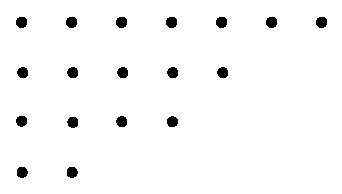
\includegraphics[scale=1.1]{figure/fig2.1.eps}
\caption{}
\end{figure}

\begin{remark}\label{chap2-rem2.1}
To solve the problem \eqref{chap2-eq2.32} by the classical approach,
one needs hard analysis involving Schauder's estimates. By the above
procedure viz.\@ the variational method, we have got through with it
more easily. 

The\pageoriginale above problem is a typical example of a second-order
problem. 
\end{remark}

\begin{exercise}\label{chap2-exer2.1}
{\em The obstacle problem}. Let $\Omega$, $\Gamma$ be as in example
\eqref{chap2-exam2.1}. Let $\mathcal{X}$ be an ``obstacle'' in this
region. Let $\mathcal{X}\leq 0$ on $\Gamma$. Let $F\,dx$ be the
density of the force acting on a membrane stretched over $\Omega$,
fixed along $\Gamma$. The displacement $u(x)$ at $x$ in the vertical
direction is the solution of the following problem:
\begin{gather*}  
\text{If}\quad V=H^{1}_{0}(\Omega),\ K=\left\{v\in H^{1}_{0}(\Omega);\
v\geq \mathcal{X}\text{~ a.e.~ in~ }\Omega\right\},\\
\text{let}\quad a(u,v)=\int_{\Omega}\sum^{n}_{i=1}\frac{\p u}{\p
  x_{i}}\frac{\p v}{\p x_{i}}dx,\ f(v)=\int_{\Omega}fv\ dx,\ f\in
L^{2}(\Omega),\\
\mathcal{X}\in H^{2}(\Omega),\ \mathcal{X}\leq 0\text{~ on~ }\Gamma.
\end{gather*}

Show that $K$ is a closed convex set and hence that this problem
admits of a unique solution. Assuming the regularity result $u\in
H^{2}(\Omega)\cap H^{1}_{0}(\Omega)$, show that this problem solves
the classical problem,
$$
\begin{cases}
u\geq \mathcal{X}\text{~ in~ } \Omega,\\
-\Delta u=f\quad\text{when}\quad u>\mathcal{X},\quad (f=F/t)\\
u=0\cdot \Gamma
\end{cases}
$$
(We will discuss the Obstacle Problem in Sec.~\ref{chap9}).
\end{exercise}

\begin{figure}[H]
\centering
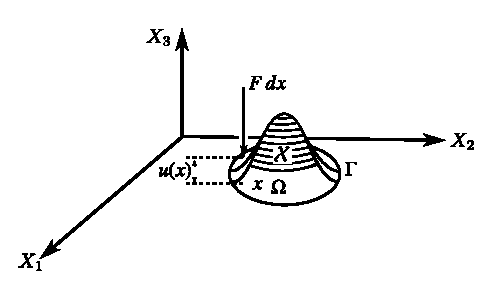
\includegraphics[scale=1.1]{figure/fig2.2.eps}
\caption{}\label{chap2-fig2.2}
\end{figure}

\begin{exercise}\label{chap2-exer2.2}
Let\pageoriginale $V=H^{1}(\Omega)$. Define $a(\cdot,\cdot)$,
$f(\cdot)$ as in example \ref{chap2-exam2.1}. Assume further that
there exists a constant $a_{0}$ such that $a\geq a_{0}>0$ in
$\Omega$. If $u_{0}$ is a given function in $H^{1}(\Omega)$, define
\begin{align*}
K &= \left\{v\in H^{1}(\Omega);\ v-u_{0}\in
H^{1}_{0}(\Omega)\right\}\\
 &= \left\{v\in
H^{1}(\Omega);\ \tr_{\Gamma}v=\tr_{\Gamma}u_{0}\right\}. 
\end{align*}

Check that $K$ is a closed convex subset. Interpret the solution to be
that of the {\em Non-homogeneous Dirichlet problem,}
\begin{equation*}
\begin{cases}
-\Delta u+au =f\quad\text{in}\quad \Omega.\\
u=u_{0}\quad\text{on}\quad \Gamma.
\end{cases}
\end{equation*}
\end{exercise}

\begin{example}\label{chap2-exam2.2}
Let $K=V=H^{1}(\Omega)$. Let $a\in L^{\infty}(\Omega)$ such that
$a\geq a_{0}>0$, $f\in L^{2}(\Omega)$. Define $a(\cdot,\cdot)$ and
$f(\cdot)$ as in example \eqref{chap2-eq2.1}. The continuity of
$a(\cdot,\cdot)$ and $f(\cdot)$ follow as usual. For the
$V$-ellipticity, we can no longer prove it with the semi-norm
$|\cdot|_{1,\Omega}$ as we did earlier. It is here we use the
additional assumption on $a$, since
\begin{align*}
a(v,v) &= \int_{\Omega}\left(\sum^{n}_{i=1}\left(\frac{\p v}{\p
  x_{i}}\right)^{2}+av^{2}\right)dx\\ 
&\geq \min (1,a_{0})||v||^{2}_{1,\Omega}.
\end{align*}

Thus we have a unique solution $u$ to the abstract problem satisfying
$a(u,v)=f(v)$. If we assume again that $u$ is ``sufficiently smooth''
to apply the Green's formula \eqref{chap2-eq2.16}, we get
\begin{equation*}
\int_{\Omega}(-\Delta u+au)v\ dx+\int_{\Gamma}\frac{\p u}{\p
  \nu}v\ d\gamma=\int_{\Gamma}fv\ dx.\tag{2.34}\label{chap2-eq2.34}
\end{equation*}

If $v\in\mathscr{D}(\Omega)$, then the integral over $\Gamma$ will
vanish. Thus $u$ satisfies the equation\pageoriginale $-\Delta u+au=f$
as in Example \ref{chap2-exam2.1}\footnote[1]{As in Example
  \ref{chap2-exam2.1}, the equation $-\Delta u+au=f$ is always
  satisfied in the sense of distributions since
  $\mathscr{D}(\Omega)\subset H^{1}(\Omega)$.}. However we now get a
different boundary condition. In example \eqref{chap2-exam2.1} the
boundary condition was built in with the assumption $u\in
V=H^{1}_{0}(\Omega)$. Now from \eqref{chap2-eq2.34}, we may write:
\begin{equation*}
\int_{\Omega}(-\Delta u+au-f)v\ dx=-\int_{\Gamma}\frac{\p u}{\p
  \nu}v\ d\gamma\tag{2.35}\label{chap2-eq2.35}
\end{equation*}
for all $v\in H^{1}(\Omega)$.

But the left hand side of \eqref{chap2-eq2.35} is zero since $u$
satisfies the differential equation as above so that for all $v\in
H^{1}(\Omega)$, $\int_{\Gamma}\frac{\p u}{\p \nu}v\ d\gamma=0$. Thus
$\dfrac{\p u}{\p \nu}=0$ on $\Gamma$, and we may interpret this
problem as the classical problem:
\begin{equation*}
\begin{cases}
-\Delta u+au=f\text{~ in~ } \Omega\\
\frac{\p u}{\p \nu}=0\text{~ on~ }\Gamma.
\end{cases}\tag{2.36}\label{chap2-eq2.36}
\end{equation*}

This is a {\em homogeneous Neumann problem.}
\end{example}

\begin{exercise}\label{chap2-exer2.3}
With $K$, $V$, $a(\cdot,\cdot)$ as in example \ref{chap2-exam2.2}.,
define
$$
f(v)=\int_{\Omega}fv\ dx+\int_{\Gamma}gv\ d\gamma,\ 
\begin{cases}
f\in L^{2}(\Omega),\\
g\in L^{2}(\Omega).
\end{cases}
$$

Show that the abstract problem leads to a solution of the {\em
  non-homo\-geneous Neumann problem}
$$
\begin{cases}
-\Delta u +au =f\text{~ in~ }\Omega\\
\dfrac{\p u}{\p \nu}=g\text{~ on~ }\Gamma.
\end{cases}
$$
\end{exercise}

\begin{remark}\label{chap2-rem2.2}
In\pageoriginale these examples one may use the more general bilinear
from defined by
\begin{equation*}
a(u,v)=\int_{\Omega}\left(\sum^{n}_{i,j=1}a_{ij}\frac{\p u}{\p
  x_{j}}\frac{\p v}{\p
  x_{i}}+auv\right)dx,\tag{2.37}\label{chap2-eq2.37} 
\end{equation*}
where the functions $a_{ij}\in L^{\infty}(\Omega)$ satisfy the
condition that for some $\nu>0$,
\begin{equation*}
\sum^{n}_{i,j=1}a_{ij}\xi_{i}\xi_{j}\geq
\nu\sum^{n}_{i=1}\xi^{2}_{i}\tag{2.38}\label{chap2-eq2.38} 
\end{equation*}
for all $\xi\in\mathbb{R}^{n}$ and a.e.\@ in $\Omega$. This is the
classical ellipticity condition for second order partial differential
operators. One should check (exercise!) in this case that the abstract
problem leads to a solution of the boundary value problem
\begin{equation*}
-\sum^{n}_{i,j=1}\frac{\p}{\p x_{i}}\left(a_{ij}\frac{\p u}{\p
  x_{j}}\right)+au=f\text{~ in~ }\Omega\tag{2.39}\label{chap2-eq2.39}
\end{equation*}
with the boundary condition
\begin{equation*}
\begin{cases}
u=0\text{~ on~ }\Gamma \text{~ if~ } K=V=H^{1}_{0}(\Omega),\\
\sum\limits^{n}_{i,j=1}a_{ij}\frac{\p u}{\p x_{j}}\nu_{i}=0\text{~ on~
}\Gamma\text{~ if~ }K=V=H^{1}(\Omega). 
\end{cases}\tag{2.40}\label{chap2-eq2.40}
\end{equation*}

The latter boundary operator in \eqref{chap2-eq2.40} is called the
{\em conormal derivative} associated with the partial differential
  operator, 
$$
-\sum^{n}_{i,j=1}\frac{\p}{\p
    x_{i}}\left(a_{ij}\dfrac{\p}{\p x_{j}}\right).
$$
 Notice that the  term ($+$ au) contributes nothing.
\end{remark}

\begin{example}\label{chap2-exam2.3}
{\em System of Elasticity.} Let $\Omega\subset \mathbb{R}^{3}$, with
Lipschitz continuous boundary $\Gamma$. Further assume that $\Gamma$
can be partitioned into two portions $\Gamma_{0}$ and $\Gamma_{1}$
such that the $d\gamma$-measure of $\Gamma_{0}$ is $>0$. Let
$$ 
K=V=\left\{\overrightarrow{v}=(v_{1},v_{2},v_{3});\ v_{i}\in
H^{1}(\Omega),\ 1\leq i\leq 3\text{ and
}\overrightarrow{v}=\overrightarrow{0}\text{ on }\Gamma_{0}\right\}.  
$$ 

Define\pageoriginale
\begin{equation*}
\begin{cases}
\epsilon_{ij}(\overrightarrow{v})=\dfrac{1}{2}\left(\dfrac{\p v_{i}}{\p
  x_{j}}+\dfrac{\p v_{j}}{\p x_{i}}\right),\\
\sigma_{ij}(\overrightarrow{v})=\lambda\left(\sum^{3}_{k=1}\epsilon_{kk}(\overrightarrow{v})\right)\delta_{ij}+2\mu
\epsilon_{ij}(\overrightarrow{v}), 
\end{cases}\tag{2.41}\label{chap2-eq2.41}
\end{equation*}
for $1\leq i$, $j\leq 3$. The latter relation is usually known as {\em
  Hooke's law}. The constants $\lambda(\geq 0)$ and $\mu(>0)$ are
known as {\em Lame's coefficients}. We define the bilinear form
$a(\cdot,\cdot)$ by,
\begin{equation*}
\begin{split}
a(\overrightarrow{u},\ora{v}) &=
\int_{\Omega}\sum^{3}_{i,j=1}\sigma_{ij}(\ora{u}\epsilon_{ij}(\ora{v})dx\\
&= \int_{\Omega}(\lambda\Div
\ora{v}+2\mu\sum^{3}_{i,j=1}\epsilon_{ij}(\ora{u})\epsilon_{ij}(\ora{v})dx. 
\end{split}\tag{2.42}\label{chap2-eq2.42}
\end{equation*}

Let $\ora{f}=(f_{1},f_{2},f_{3})$, $f_{i}\in L^{2}(\Omega)$, and
$\ora{g}=(g_{1},g_{2},g_{3})$, $g_{i}\in L^{2}(\Gamma)$, be given.

Define the linear functional $f(\cdot)$, by,
\begin{equation*}
f(\ora{v})=\int_{\Omega}\ora{f}\cdot
\ora{v}dx+\int_{\Gamma_{1}}\ora{g}\cdot\ora{v}d\gamma.\tag{2.43}\label{chap2-eq2.43} 
\end{equation*}

The continuity of $a(\cdot,\cdot)$ and $f(\cdot)$ follow from the
Cauchy-Schwarz inequality. For the $V$-ellipticity of $a(\cdot,\cdot)$
one uses the inequality
$$
a(\ora{v},\ora{v})\geq
2\mu\int_{\Omega}\sum^{3}_{i,j=1}(\epsilon_{ij}(\ora{v}))^{2}dx 
$$
and the fact that the square root of the integral appearing in the
right hand side of the above inequality is a norm over the space $V$,
equivalent to the norm $\ora{v}=(v_{1},v_{2},v_{3})\mapsto
(\sum^{3}_{i=1}||v_{i}||^{2}_{1,\Omega})^{\frac{1}{2}}$. This is a
nontrivial fact which uses essentially the fact that $\Gamma_{0}$ has
measure $>0$ and an inequality known as {\em K\"orn's inequality}. We
omit the proof here.

Again the problem $a(\ora{u},\ora{v})=f(\ora{v})$ admits a unique
solution. Assuming\pageoriginale sufficient smoothness, we may apply
Green's formula:
\begin{align*}
\int_{\Omega}\sum^{3}_{i,j=1}\sigma_{ij}(\ora{u})\epsilon_{ij}(\ora{v})dx
&=
\frac{1}{2}\int_{\Omega}\sum^{3}_{i,j=1}\sigma_{ij}(\ora{u})\left(\frac{\p
  v_{i}}{\p x_{j}}+\frac{\p v_{j}}{\p x_{i}}\right)dx\\
&= \int_{\Omega}\sum^{3}_{i,j=1}\sigma_{ij}(\ora{u})\frac{\p v_{i}}{\p x_{j}}dx
\end{align*}
(since $\epsilon_{ij}(v)$ is symmetric in $i$ and $j$)
$$
=-\int_{\Omega}\sum^{3}_{i,j=1}\frac{\p}{\p x_{j}}(\sigma_{ij}(\ora{u}))v_{i}dx+\int_{\Gamma_{1}}\sum^{3}_{i,j=1}\sigma_{ij}v_{i}\nu_{j}d\gamma.
$$

Thus, the abstract problem leads to a solution of
\begin{equation*}
\begin{cases}
-\sum\limits^{3}_{j=1}\frac{\p}{\p x_{j}}(\sigma_{ij}(\ora{u}))=f_{i}(1\leq
i\leq 3)\text{~ in~ }\Omega\\
\qquad \ora{u}=\ora{0}\text{~ on~ }\Gamma_{0}\text{~ and}\\
\sum\limits^{3}_{j=1}\sigma_{ij}(\ora{u})\nu_{j}=g_{i}\text{~ on~
}\Gamma_{1}(1\leq i\leq 3).
\end{cases}\tag{2.44}\label{chap2-eq2.44}
\end{equation*}

Note also that
{\fontsize{10}{12}\selectfont
\begin{align*}
-\sum^{3}_{j=1}\frac{\p}{\p x_{j}}(\sigma_{ij}(\ora{u})) & =
-\sum^{3}_{j=1}\frac{\p}{\p x_{j}}\left(\lambda
\sum^{3}_{k=1}\epsilon_{kk}(\ora{u})\delta_{ij}+2\mu
\epsilon_{ij}(\ora{u})\right)\\ 
&= -\sum^{3}_{j=1}\frac{\p}{\p
x_{j}}\left(\lambda\sum^{3}_{k=1}\frac{\p u_{k}}{\p
x_{k}}\right)\delta_{ij}-\sum^{3}_{j=1}\frac{\p}{\p
x_{j}}\left(2\mu\left(\frac{\p u_{i}}{\p x_{j}}+\frac{\p u_{j}}{\p
x_{i}}\right)\right)\\
&= -(\lambda+\mu)(\text{grad~ }\Div\ora{v})_{i}-\mu\Delta u_{i}. 
\end{align*}}

Thus the first equation of \eqref{chap2-eq2.44} is equivalent to
\begin{equation*}
-\mu\Delta \ora{u}-(\lambda+\mu)\grad \Div \ora{u}=\ora{f}\text{~ in~
}\Omega.\tag{2.45}\label{chap2-eq2.45}
\end{equation*}

The equations \eqref{chap2-eq2.44} constitute the {\em system of
  linear Elasticity.}
\begin{figure}[H]
\centering
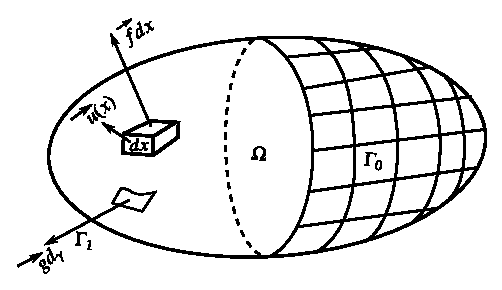
\includegraphics{figure/fig2.3.eps}
\caption{}\label{chap2-fig2.3}
\end{figure}\pageoriginale 

If we have an elastic three-dimensional body fixed along $\Gamma_{0}$,
acted on by an exterior force of density $f\,dx$ and force of density
$g\,d\gamma$ along $\Gamma_{1}$ and if $\sigma_{ij}$ is the stress
tensor, the displacement $u$ satisfies \eqref{chap2-eq2.44}; cf.\@
Fig.~\ref{chap2-fig2.3}. 

The relation $a(\ora{u},\ora{v})=f(\ora{v})$, viz.,
\begin{equation*}
\int_{\Omega}\sum^{3}_{i,j=1}\sigma_{ij}(\ora{u})\epsilon_{ij}(\ora{v})dx=\int_{\Omega}\ora{f}\cdot\ora{v}dx+\int_{\Gamma_{1}}\ora{g}\cdot\ora{v}d\gamma\tag{2.46}\label{chap2-eq2.46} 
\end{equation*}
for all $\ora{v}\in V$ is known as the {\em principle of virtual
  work}. The tensor $\epsilon_{ij}$ is {\em the strain tensor} and the
tensor $\sigma_{ij}$ {\em the stress tensor}. The expression
$\frac{1}{2}a(\ora{v},\ora{v})$ is the {\em strain energy}, and the
functional $f(\ora{v})$ is the {\em potential energy of exterior
  forces.} This example is of fundamental importance in that the
finite element method has been essentially developed for solving this
particular problem or some of its special cases (membranes, plates,
shells, etc.,) and generalizations (nonlinear elasticity, etc\ldots).
\end{example}

\eject

\begin{remark}\label{chap2-rem2.3}
The\pageoriginale above problems are all examples of {\em linear
  problems}\footnote[2]{Except in Exercise \ref{chap2-exer2.1}.}:
The map from the right-hand side of the equation and of the boundary
conditions to the solution $u$ is linear. The non-linearity may occur
in three ways:
\begin{itemize}
\item[(i)] When $K$ is not a subspace of $V$. (e.g. Exercises
  \ref{chap2-exer2.1} and \ref{chap2-exer2.4}); 

\item[(ii)] If in Example \ref{chap2-exam2.3} we have, instead of the
  first equality in \eqref{chap2-eq2.41}:
$$
\epsilon_{ij}(\ora{v})=\frac{1}{2}\left[\left(\frac{\p v_{i}}{\p
    x_{j}}+\frac{\p v_{j}}{\p x_{i}}\right)+\sum^{3}_{k=1}\frac{\p
    v_{k}}{\p x_{i}}\frac{\p v_{k}}{\p x_{j}}\right].  
$$

This is the case for instance when one derives the so-called Von
Karmann's equations of a clamped plate;

\item[(iii)] We may replace Hooke's law (the second relations in
  \eqref{chap2-eq2.41}) by non-linear equations connecting
  $\epsilon_{ij}$ and $\sigma_{ij}$, which are known as {\em
    non-linear constitutive equations}. (e.g.\@ {\em Hencky's law}). 
\end{itemize}
\end{remark}

\begin{exercise}\label{chap2-exer2.4}
Let $V=H^{1}(\Omega)$, and $a(\cdot,\cdot)$ and $f(\cdot)$ be as in
example \ref{chap2-exam2.2}, and let
{\fontsize{10}{12}\selectfont
$$
K=\left\{v\in H^{1}(\Omega);\ v\geq 0\text{~ a.e.~ on~ }
\Gamma\right\}.
$$}

Show that $K$ is a closed convex cone with vertex $0$. Using the
results of Sec.~\ref{chap1} show that the interpretation is
\begin{gather*}
-\Delta u+au=f\text{~ in~ }\Omega,\\
u\geq 0,\ \frac{\p u}{\p \nu}\geq 0,\ u\frac{\p u}{\p \nu}=0\text{~
  on~ } \Gamma.
\end{gather*}
(This is called the {\em SIGNORINI problem}).
\end{exercise}

We now examine fourth-order problems.

\begin{example}\label{chap2-exam2.4}
Let $K=V=H^{2}_{0}(\Omega)$. Define 
\begin{equation*}
\begin{cases}
a(u,v)=\int_{\Omega}\Delta u\Delta v\ dx,\\
f(v)=\int_{\Omega}fv\ dx,\ f\in L^{2}(\Omega),
\end{cases}\tag{2.47}\label{chap2-eq2.47}
\end{equation*}\pageoriginale
for all $u$, $v\in V$. The continuity follows as usual. For the
$V$-ellipticity of $a(\cdot,\cdot)$ we have,
\begin{equation*}
a(v,v)=\int_{\Omega}(\Delta v)^{2}dx=|\Delta
v|^{2}_{0,\Omega}=|v|^{2}_{2,\Omega}.\tag{2.48}\label{chap2-eq2.48} 
\end{equation*}
(by Lemma \ref{chap2-lem2.1}. Since $|\cdot|_{2,\Omega}$ and $||\cdot
||_{2,\Omega}$ are equivalent on $H^{2}_{0}(\Omega)$, the
$V$-ellipticity follows from \eqref{chap2-eq2.48}.

Hence there exists a unique function $u\in H^{2}_{0}(\Omega)$ such
that
\begin{equation*}
\int_{\Omega}\Delta u\Delta v\ dx=\int_{\Omega}fv\ dx\text{~ for all~
} v\in H^{2}_{0}(\Omega).
\end{equation*}

Assuming $u$ to be sufficiently smooth (say, $u\in H^{4}(\Omega)$),
then by Green's formula \eqref{chap2-eq2.18},
\begin{equation*}
\int_{\Omega}(\Delta^{2}u-f)v\ dx=\int_{\Gamma}\frac{\p (\Delta u)}{\p
  \nu}v\ d\gamma-\int_{\Gamma}\Delta u\frac{\p v}{\p
  \nu}d\gamma,\tag{2.50}\label{chap2-eq2.50} 
\end{equation*}
for all $v\in H^{2}_{0}(\Omega)$. Hence by varying $v$ over
$H^{2}_{0}(\Omega)$, we get that $u$ satisfies $\Delta^{2}u=f$ in
$\Omega$. Since $u\in H^{2}_{0}(\Omega)$, the boundary conditions are
given by \eqref{chap2-eq2.14}. Thus we interpret this problem as the
classical problem
\begin{equation*}
\begin{cases}
\Delta^{2}u=f\text{~ in~ }\Omega,\\
u=\dfrac{\p u}{\p \nu}= 0\text{~ on~ }\Gamma.
\end{cases}\tag{2.51}\label{chap2-eq2.51}
\end{equation*}

This is the {\em homogeneous Dirichlet problem} for the operator
$\Delta^{2}$. 

When $n=2$, this is an important problem in Hydrodynamics. Here $u$ is
known as the stream function and $-\Delta u$ is the {\em vorticity}.


A\pageoriginale slight modification of $a(\cdot,\cdot)$ leads to an
important problem in Elasticity. Again let $n=2$. Let $f\in
L^{2}(\Omega)$ and if $K=V=H^{2}_{0}(\Omega)$, define 
{\fontsize{9}{11}\selectfont
\begin{equation*}
\begin{cases}
f(v)=\int_{\Omega}fv\ dx,\\
a(u,v)=\int_{\Omega}\left[\Delta u\ \Delta
  v+(1-\sigma)\left(2\dfrac{\p^{2}u}{\p x_{1}\p x_{2}}\dfrac{\p^{2}v}{\p
    x_{1}\p x_{2}}-\dfrac{\p^{2}u}{\p x^{2}_{1}}\dfrac{\p^{2}v}{\p
    x^{2}_{2}}-\dfrac{\p^{2}u}{\p x^{2}_{2}}\dfrac{\p^{2}v}{\p
    x^{2}_{1}}\right)\right]dx. 
\end{cases}\tag{2.52}\label{chap2-eq2.52}
\end{equation*}}

The integrand occurring in the definition of $a(u,v)$ may also be
written as
\begin{equation*}
\sigma \Delta u\Delta v+(1-\sigma)\left(\frac{\p^{2}u}{\p
  x^{2}_{1}}\frac{\p^{2}v}{\p x^{2}_{1}}+\frac{\p^{2}u}{\p
  x^{2}_{2}}\frac{\p^{2}v}{\p x^{2}_{2}}+\frac{2\p^{2}u}{\p x_{1}\p
  x_{2}}\frac{\p^{2}v}{\p x_{1}\p
  x_{2}}\right). \tag{2.53}\label{chap2-eq2.53} 
\end{equation*}

{\em Usually, from physical considerations}, $0<\sigma<\dfrac{1}{2}$.

Note that
\begin{equation*}
a(v,v)=\sigma|\Delta
v|^{2}_{0,\Omega}+(1-\sigma)|v|^{2}_{2,\Omega}\tag{2.54}\label{chap2-eq2.54} 
\end{equation*}
by \eqref{chap2-eq2.53} and this leads to the $V$-ellipticity of
$a(\cdot,\cdot)$. By virtue of \eqref{chap2-eq2.21} in Lemma
\ref{chap2-lem2.2}, we get that the relations $a(u,v)=f(v)$ read as
\begin{equation*}
\int_{\Omega}\Delta^{2}uv\ dx=\int_{\Omega}fv\ dx,\tag{2.55}\label{chap2-eq2.55} 
\end{equation*}
assuming sufficient smoothness of $u$. Thus again we get the same
equation as in \eqref{chap2-eq2.51}. Notice that the additional term
in the definition of $a(\cdot,\cdot)$ has contributed nothing towards
the differential equation.

This latter problem is known as the {\em clamped plate problem}: 

Consider a plate of ``small'' thickness $e$ lying on the
$x_{1}x_{2}$-plane. Let $E$ be its Young's modulus and $\sigma$ its
Poisson coefficient. Let there be a load $F$ acting on the plate. The
displacement $u$ is the solution of \eqref{chap2-eq2.51}, where $f$ is
given by (cf. Fig.~\ref{chap2-fig2.4}):
\begin{equation*}
F=\frac{E e^{3}f}{12(1-\sigma^{2})}.\tag{2.56}\label{chap2-eq2.56}
\end{equation*}\pageoriginale
\end{example}
\begin{figure}[H]
\centering
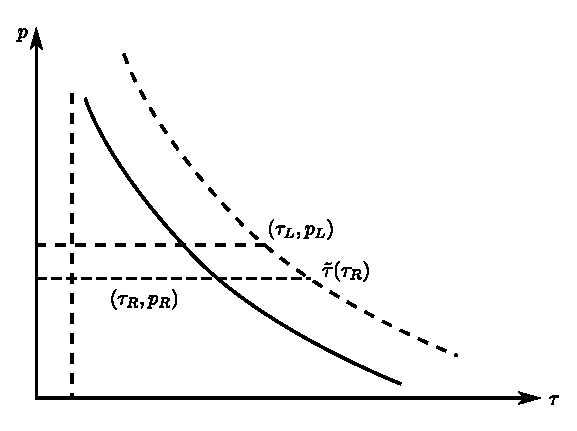
\includegraphics{figure/fig2.4.eps}
\caption{}\label{chap2-fig2.4}
\end{figure}

We will return to this problem in Sections 10 and 11.

\begin{exercise}\label{chap2-exer2.5}
Let $K=V=\{v\in H^{2}(\Omega);\ v=0\text{~ on~
}\Gamma\}=H^{2}(\Omega)\cap H^{1}_{0}(\Omega)$, and define
$a(\cdot,\cdot)$ and $f(\cdot)$ as in the case of the clamped
plate. Assuming the $V$-ellipticity of $a(\cdot,\cdot)$ show that the
solution of the abstract problem satisfies $\Delta^{2}u=f$ in $\Omega$
and $u=0$ on $\Gamma$. What is the other boundary condition? This is
known as the problem of the {\em simply supported plate.}
\end{exercise}

\begin{exercise}\label{chap2-exer2.6}
Let $K=V=H^{2}(\Omega)\cap H^{1}_{0}(\Omega)$, and
\begin{align*}
a(u,v) &= \int_{\Omega}\Delta u\Delta v\ dx;\\
f(v) &= \int_{\Omega}fv\ dx-\int_{\Gamma}\lambda\dfrac{\p v}{\p
  \nu}d\gamma,\text{~ where~ } f\in L^{2}(\Omega),\ \lambda \in
L^{2}(\Gamma). 
\end{align*}

Show that we may apply the result of Sec.~\ref{chap1} and give an
interpretation of this problem.
\end{exercise}

\noindent
{\bf REFERENCES.}~ For details on Sobolev spaces, see Ne\v{c}as
\cite{key20} and Lions and Magenes \cite{key17}. For the theory of
Elasticity, one may refer to Duvaut and Lions \cite{key10} and Landau
and Lipschitz \cite{key14}.
